\section{Use Cases der Applikation}
\label{Use Case Diagramme}
Aus dem Lastehheft selbst und aus dessen Auswertung, ergeben sich f\"ur den Nutzer der App gewisse Use-Cases, welche in den folgenden Use Case Diagrammen genauer beschrieben werden.

Im Use Case Diagramm im Bild \ref{Main Use Case} ist links der Nutzer der App dargestellt. Er hat innerhalb der App die f\"unf Use Cases Alarmierung, Regelerstellung, Alarmeinstellung, Ger\"atehauseinstellung und Regel versenden. Bei der Regelerstellung kann der Nutzer Regeln nach den Vorgaben des Lastenhefts erstellen. Zus\"atzlich hat er die M\"oglichkeit globale Alarmeinstellungen vorzunehmen und Einstellungen zum Ger\"atehaus zu treffen. Schlie\ss{}lich kann er aber auch seine erstellten Regeln an andere Nutzer versenden. 
Die Alarmierung erfolgt durch eine Leitstelle oder einen anderen Nutzer, welcher im Bild \ref{Main Use Case} rechts dargestellt ist.

Im folgenden werden nun die einzelnen Use-Cases noch einmal verfeinert aufgezeigt.
\begin{figure}[!ht]
\centering
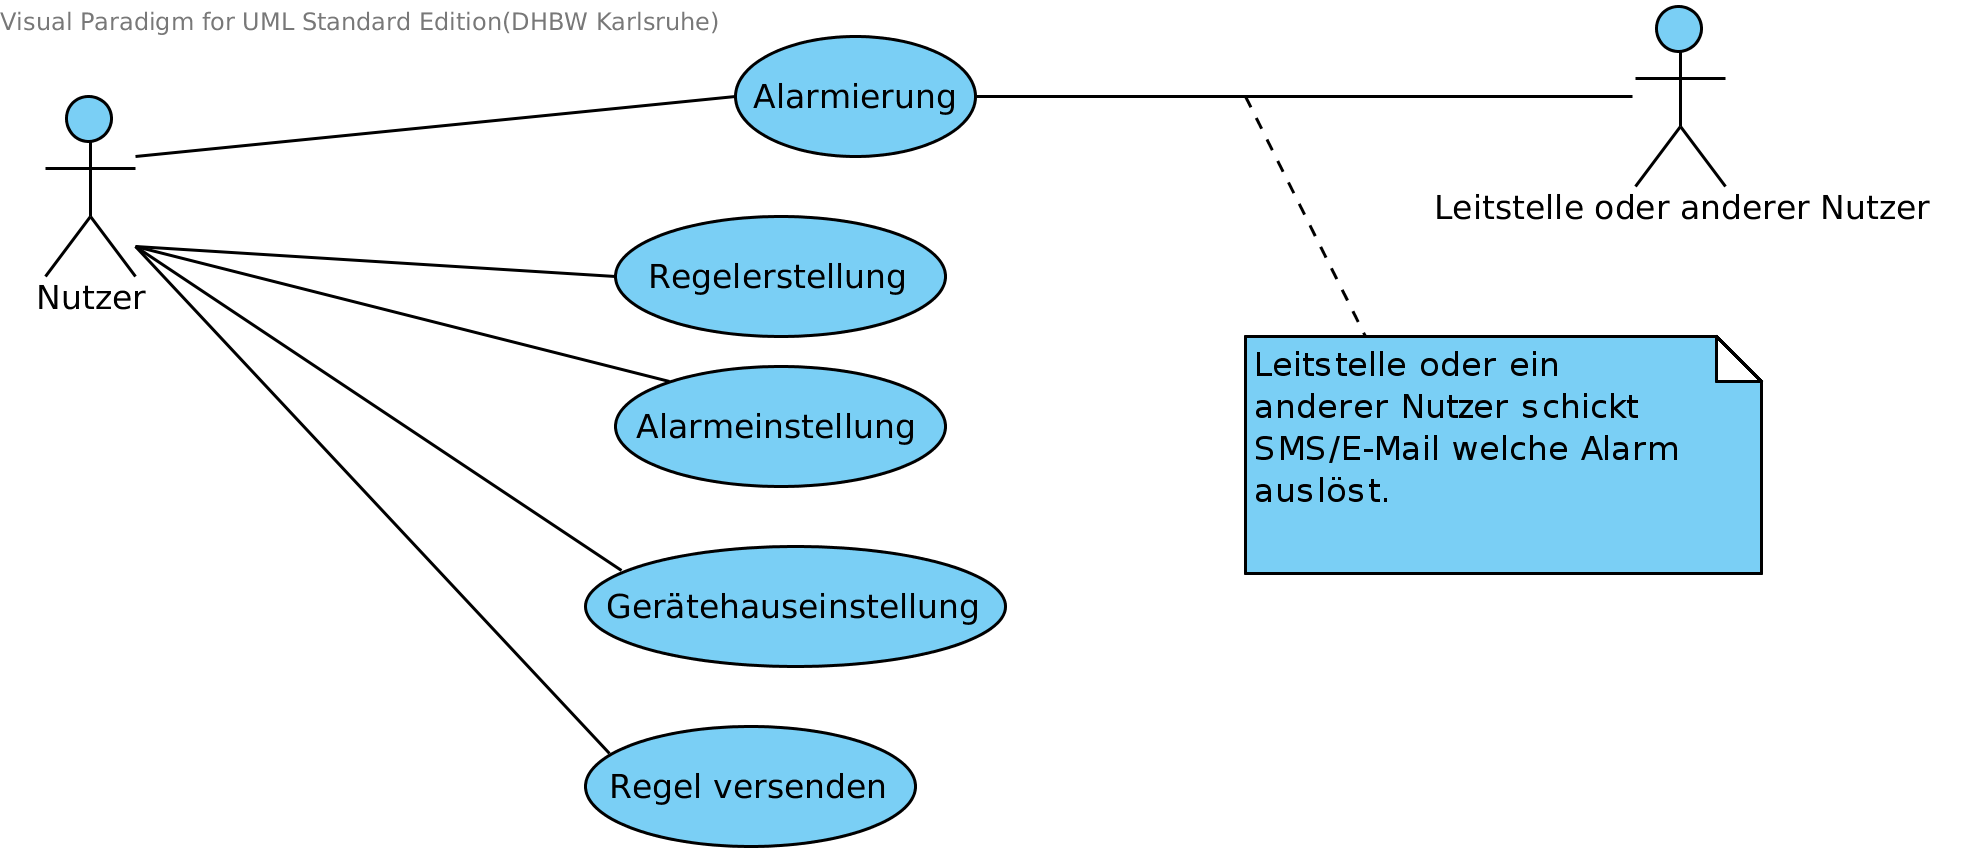
\includegraphics[width=16cm]{Bilder/AlarmSMS_App.png}
\caption{Use-Case-Diagramm der App}
\label{Main Use Case}
\centering
\end{figure}

Im Bild \ref{Regelerstellung Use Case} ist der Use-Case der Regelerstellung einmal verfeinert dargestellt. Der Nutzer hat die aufgezeigten M\"oglichkeiten bei der Regelerstellung, wie sie im Lastenheft verankert sind. Es kann ein Regelname und ein Absender ausgew\"ahlt werden. Bei der Wahl des Alarmtons, werden zus\"atzlich noch die Systemt\"one geladen und zur Auswahl gestellt. Wichtig ist nat\"urlich auch die Auswahl der Eingangsart, welche dar\"uber entscheidet, ob die Regel f\"ur eine SMS oder eine E-Mail gilt. 

Beim Hinzuf\"ugen von Schlagworten hat der Nutzer die M\"oglichkeit, W\"orter hinzuzuf\"ugen, welche enthalten sein m\"ussen, beziehungsweise welche nicht vorhanden sein d\"urfen. 

Um einen Post in einem Social Network zu machen, muss der Nutzer einen Text eingeben, welcher gepostet werden soll. Zum anderen muss die jeweilige App auf dem Ger\"at installiert sein, damit \"uber sie gepostet werden kann.

Als abschlie\ss{}enden Punkt, kann der Nutzer automatisch eine weiterf\"uhrende Benachrichtigung automatisch senden lassen, um zum Beispiel mitzuteilen, dass er nicht am Einsatz teilnimmt.
\begin{figure}[!ht]
\centering
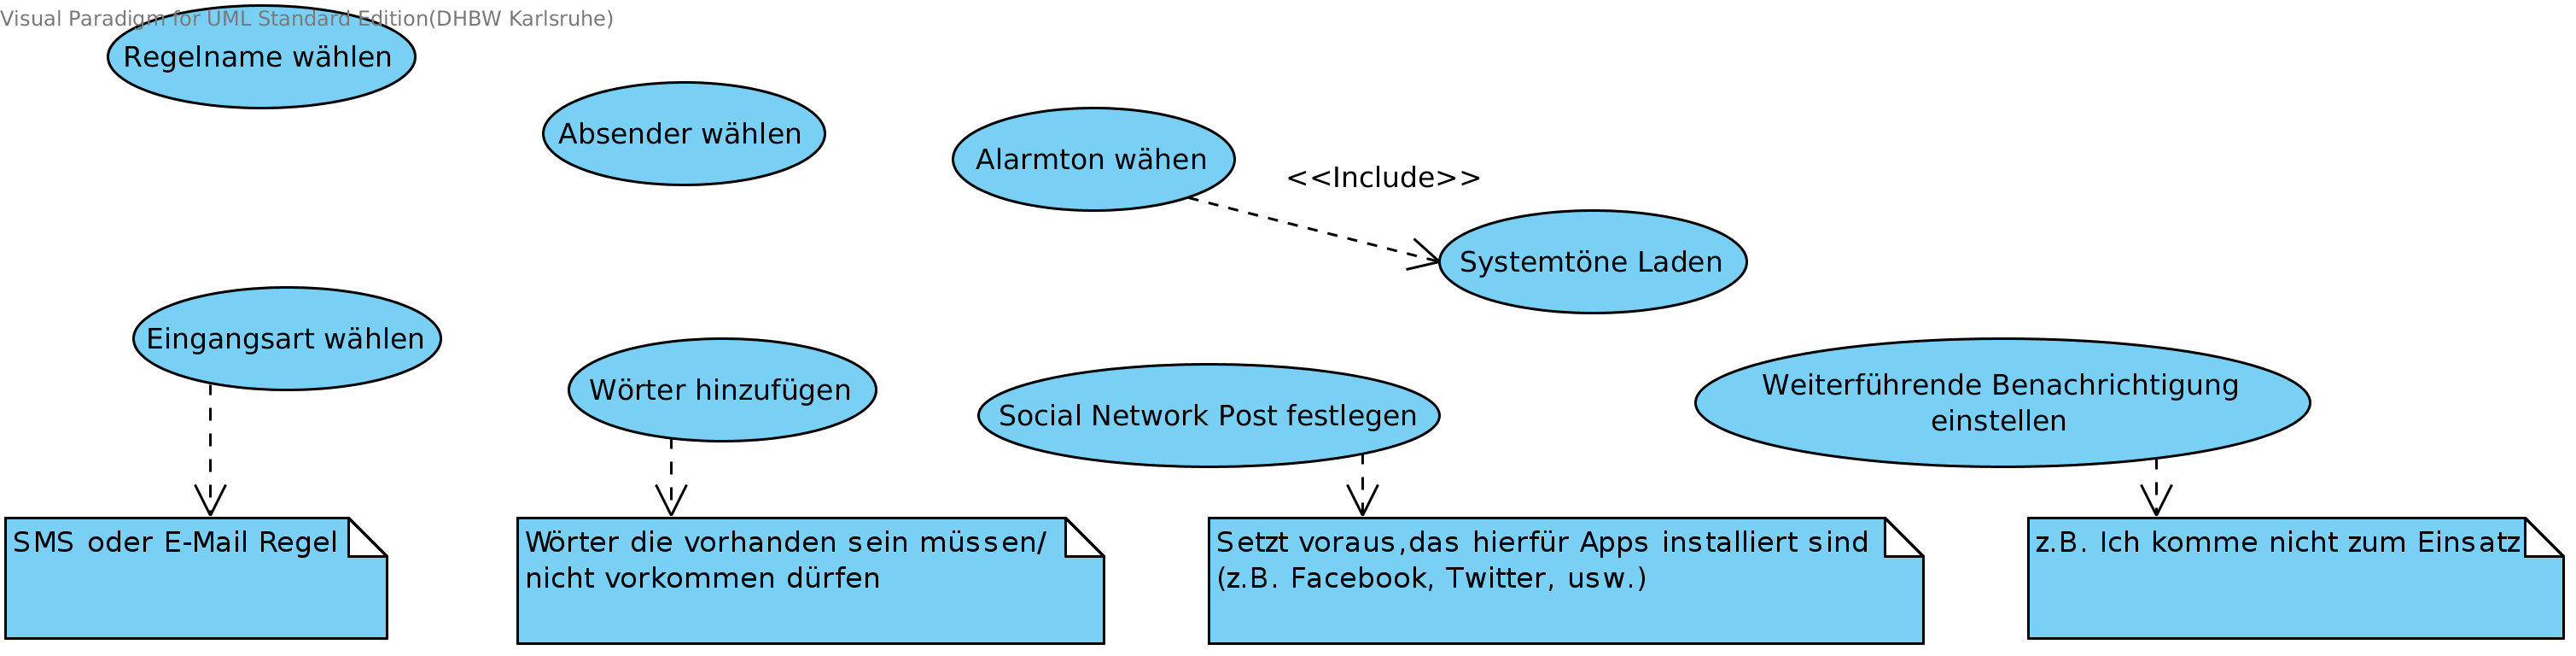
\includegraphics[width=16cm]{Bilder/UseCaseRegelerstellung.png}
\caption{Use-Case-Verfeinerung der Regelerstellung}
\label{Regelerstellung Use Case}
\centering
\end{figure}

\FloatBarrier
Im Bild \ref{Regelerstellung Use Case} ist die Alarmeinstellung als Use-Case-Verfeinerung einmal genauer dargestellt. Der Nutzer hat die M\"oglichkeit, die Alarmierung komplett zu aktivieren beziehungsweis zu deaktivieren. Sollte eine Alarmierung erfolgen, stehen weitere Einstellungsm\"oglichkeiten zur Verf\"ugung, so zum Beispiel die Aktivierung des Notificationlights und dessen Farbe. Zus\"atzlich l\"asst sich aber auch ein Vibrationsalarm einstellen.

\begin{figure}[!ht]
\centering
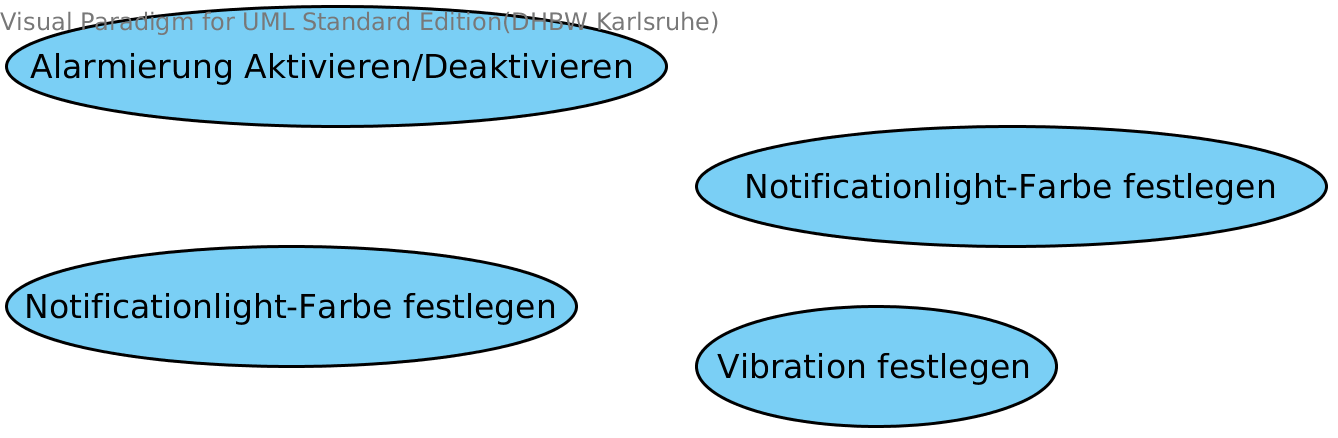
\includegraphics[width=10cm]{Bilder/UseCaseAlarmeinstellung.png}
\caption{Use-Case-Verfeinerung der Alarmeinstellung}
\label{Alarmeinstellung Use Case}
\centering
\end{figure}
Beim Use-Case der Ger\"atehauseinstellung gibt es zum einen die Auswahl eines Namens und zum anderen die Festlegung des Standortes. Die Standortbestimmung, kann zus\"atzlich mit der Unterst\"utzung von Google geschehen, wie im Bild \ref{Geraetehauseinstellung Use Case} gezeigt wird.
\begin{figure}[!ht]
\centering
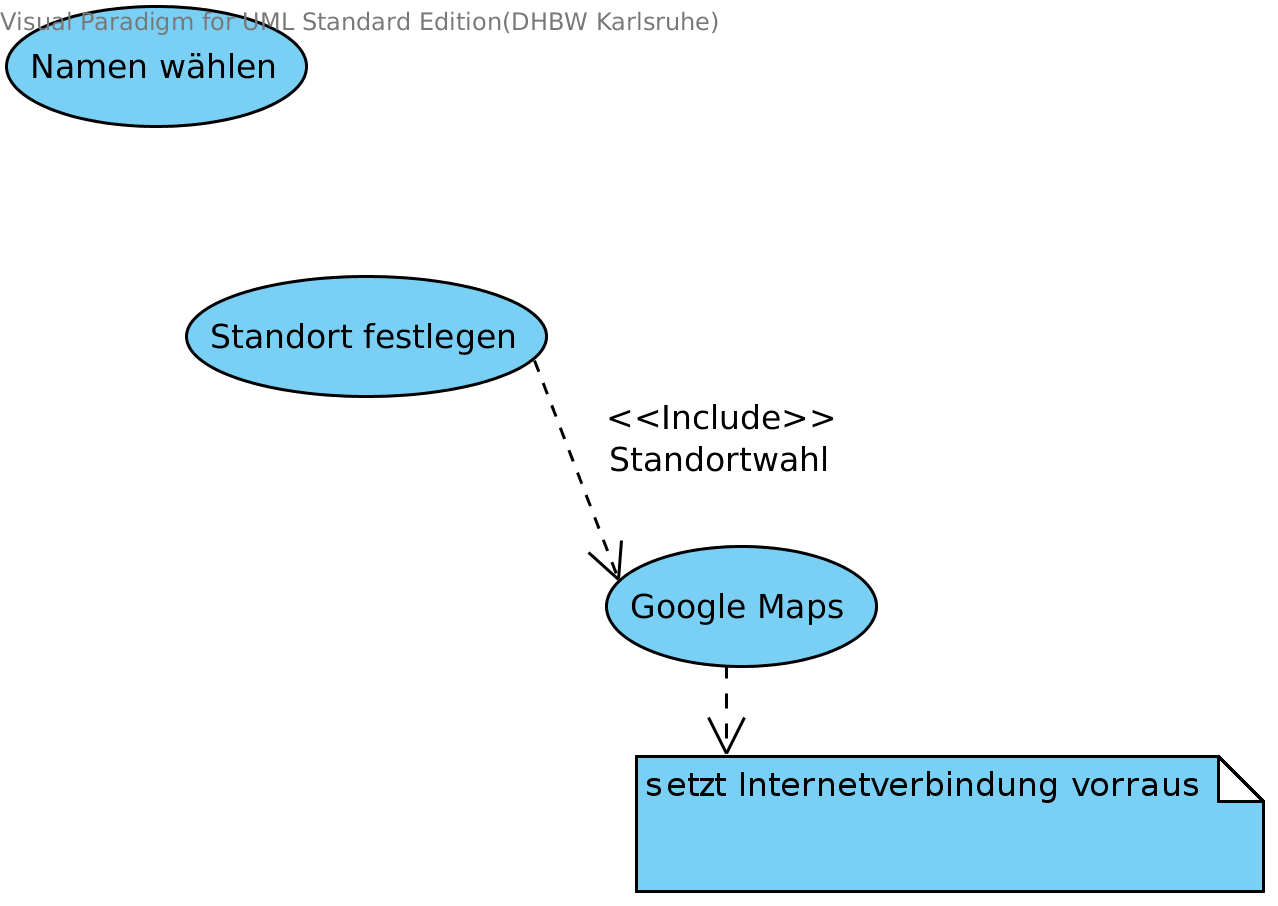
\includegraphics[width=10cm]{Bilder/UseCaseGeraetehauseinstellung.png}
\caption{Use-Case-Verfeinerung der Ger\"atehauseinstellung}
\label{Geraetehauseinstellung Use Case}
\centering
\end{figure}

\newpage

Bild \ref{Regelversendung Use Case} zeigt die Use-Case-Verfeinerung f\"ur den Fall einer Regelversendung. Im folgenden muss ein Empf\"anger gew\"ahlt werden, was beinhaltet, dass eine Kopplung zum Empf\"angerger\"at hergestellt wird. Danach muss der Nutzer eine Regel zum Versand ausw\"ahlen und diese dann versenden. 
\begin{figure}[!ht]
\centering
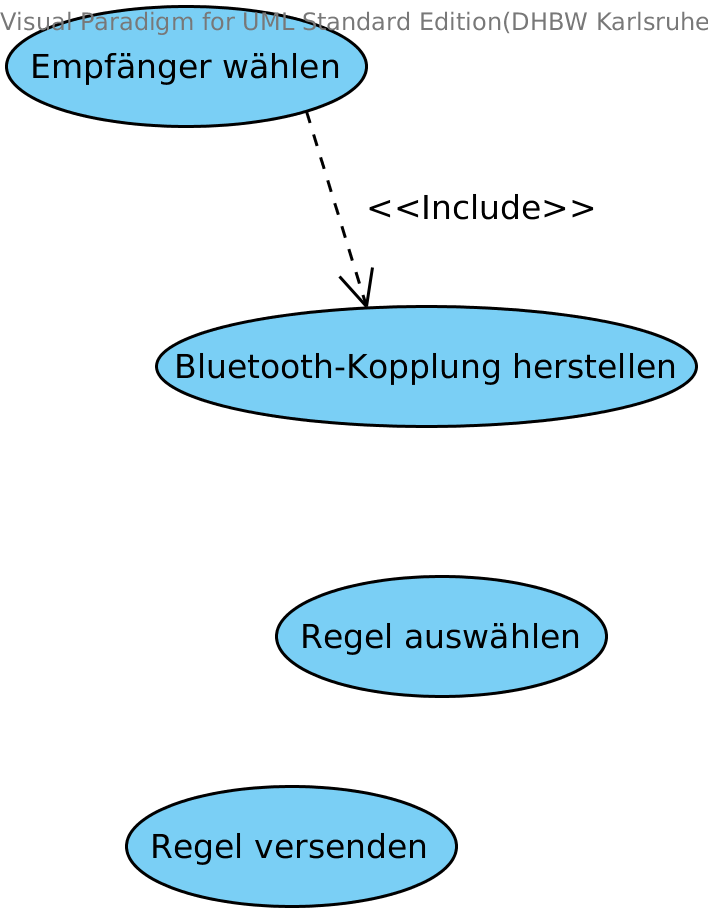
\includegraphics[width=6cm]{Bilder/UseCaseRegelVersenden.png}
\caption{Use-Case-Verfeinerung der Regelversendung}
\label{Regelversendung Use Case}
\centering
\end{figure}

Das Herzst\"uck der App ist jedoch die Alarmierung, welche im Bild \ref{Alarmierung Use Case} genauer dargestellt ist. Beim Eingehen einer Benachrichtigung wird diese gepr\"uft, was beinhaltet, dass der Empf\"anger und der Inhalt gepr\"uft wird. Sollte ein Alarmierungsfall vorliegen, so wird eine Alarmierung nach den Einstellungen des Nutzers vorgenommen. Gleichzeitig wird gegebenenfalls ein Social Network Post abgesetzt und eine weiterf\"uhrende Benachrichtigung abgesendet.
\begin{figure}[!ht]
\centering
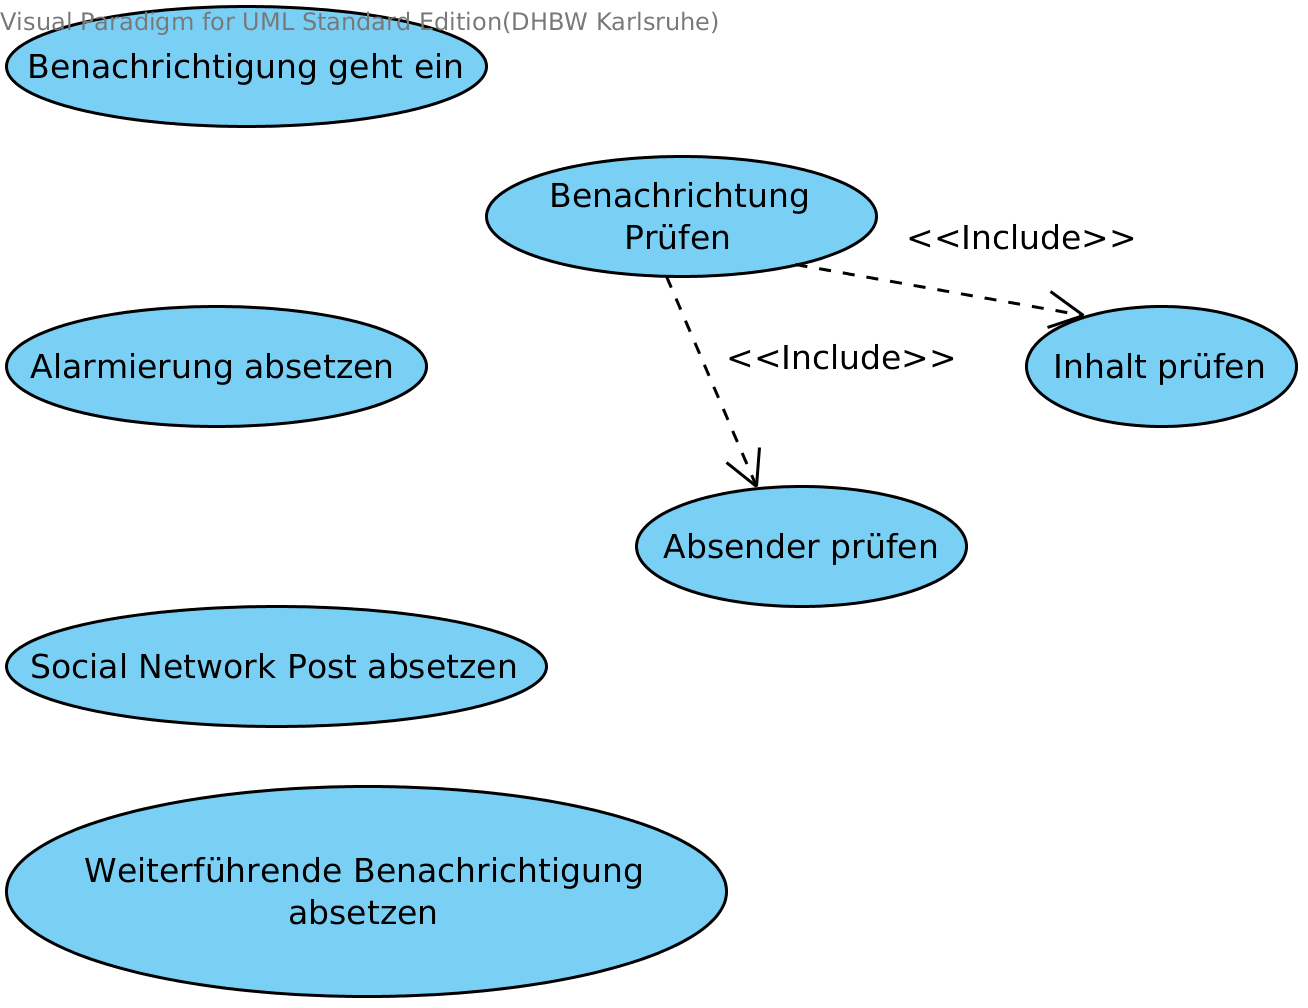
\includegraphics[width=10cm]{Bilder/UseCaseAlarmierung.png}
\caption{Use-Case-Verfeinerung der Alarmierung}
\label{Alarmierung Use Case}
\centering
\end{figure}

Aufgrund dieser Use-Cases und der Lasteheftanalyse wird im n\"achsten Kapitel auf die erstellten Wireframes eingegangen.